\section{Sonuçlar}
\label{sec:results}

\subsection{Yavaş ve Güçlü Çözücüler Hızlı Bir Sezgisel Yönteme Yenilir}
\label{sec:res_aging}
Bu senaryoda sinyalin büyük kısmını RIS taşır: doğrudan bağlantılar engellenmişken, kullanıcı başına medyan sinyal-gürültü oranı (SNR) yalnızca doğrudan bağlantı için 20.0~dB, RIS üzerinden ise 31.1~dB'dir. RIS olmadan en düşük kullanıcı hızı 1.744~b/s/Hz'dir; rastgele bir faz 4.072 verir.

Şekil~\ref{fig:aging}, her yöntemin fazını $t=0$ anında sabitler ve kullanıcılar yürürken en düşük hızı izler. Hızlar birkaç milisaniye boyunca korunur, $T_c$ civarında keskin biçimde düşer ve bayat tabanın üzerinde dengelenir. Bir faz ne kadar iyi optimize edilmişse o kadar çok kaybeder: $T_c$ anına gelindiğinde uzun koşulu Adam 7.117'den 5.473~b/s/Hz'e düşerken SU-average yalnızca 4.624'ten 4.503'e kayar.

Tablo~\ref{tab:aging}, her yöntemi kendi gecikmesinde değerlendirir. Uzun koşulu Adam ve koordinat inişi tablodaki en iyi $t=0$ hızlarına sahiptir, ancak sırasıyla 5.9~s ve 0.88~s gerektirir. O zamana kadar kullanıcılar birkaç metreye varan mesafeler kat etmiş olur ve iyimser etkin hızları bile 2.5~ms süren SU-best-of'unkinin altına düşer: SU-best-of, koordinat inişinin 0.297~b/s/Hz (\%95 GA 0.204--0.390), uzun koşulu Adam'ın ise 0.604 (0.415--0.805) önündedir. Bu, sabit bir bütçenin yapay bir sonucu değildir: tek bir çok kullanıcılı koordinat taraması zaten 107~ms, yani yaklaşık dört eş evrelilik süresi sürer ve bir ila sekiz tarama arasının en iyisi (5.014~b/s/Hz, iki tarama) SU-best-of'un 0.26~b/s/Hz altında kalır (GA 0.17--0.36).

\begin{table}[t]
\centering
\caption{$t=0$ anındaki hız, gecikme ve etkin hız (eskime kümesi, 400 senaryo, 1.5~m/s). Bayat taban: $t=0$ fazının bağımsız bir kanal üzerinde kullanılması. $^\dagger$200~ms'lik güvenilir ufkun ötesinde; iyimser. $^\ast$Son ızgara noktasındaki (5.6~s) değer.}
\label{tab:aging}
\footnotesize
\begin{tabular}{lrrrr}
\toprule
Yöntem & $t{=}0$ & Gecikme & Etkin & Bayat \\
 & (b/s/Hz) & (ms) & (b/s/Hz) & (b/s/Hz) \\
\midrule
RIS yok (doğrudan yol) & 1.744 & -- & -- & -- \\
Rastgele faz & 4.072 & -- & -- & -- \\
SU-average & 4.624 & 0.42 & 4.623 & 4.315 \\
SU-best-of & 5.276 & 2.5 & 5.272 & 4.336 \\
Adam, $L=8$ & 6.443 & 13.3 & 5.849 & 4.326 \\
Adam, $L=12$ & 6.631 & 20.0 & 5.515 & 4.370 \\
Adam, $L=16$ & 6.754 & 26.6 & 5.324 & 4.381 \\
Adam, $L=20$ & 6.835 & 33.2 & 5.276 & 4.364 \\
Koord. inişi & 6.925 & 880.8 & 4.975$^\dagger$ & 4.352 \\
Uzun koşulu Adam & 7.117 & 5851.7 & 4.667$^\dagger$$^\ast$ & 4.423 \\
\bottomrule
\end{tabular}

\end{table}

\begin{figure}[t]
\centering
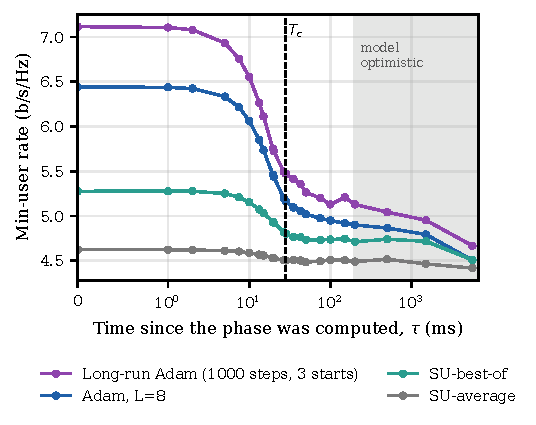
\includegraphics[width=0.92\columnwidth]{figures/fig_aging.pdf}
\caption{Kullanıcılar 1.5~m/s hızla yürürken, ön kodlayıcı tazelenerek, $t=0$ anında sabitlenen bir fazın en düşük kullanıcı hızı. Kesikli: $T_c=28.2$~ms. Gölgeli: 200~ms'nin ötesinde model iyimserdir.}
\label{fig:aging}
\end{figure}

\subsection{Birkaç Adımdan Sonra Ek Yinelemeler Yararlı Olmaktan Çıkar}
\label{sec:res_optimum}
Şekil~\ref{fig:optimum}, Adam adım sayısını SU-average'dan (4.624~b/s/Hz) başlayarak tarar. $t=0$ hızı her adımda artar: $L=1$'de 5.412'den $L=48$'de 7.037~b/s/Hz'e. Etkin hız ise artmaz: $L=4$--$6$'da tepe yapar (6.7--10.0~ms'de 5.980, 5.982 ve 5.970~b/s/Hz) ve diğer her adım sayısı anlamlı ölçüde daha düşüktür. $L=48$'de, oradaki $t=0$ hızı \%13.2 daha yüksek olmasına rağmen, etkin hız tepenin \%14.0 (\%95 GA \%12.5--15.5) altındadır. \eqref{eq:marginal} ifadesi açısından, $L=4$'ten $6$'ya geçmek $t=0$ anında 0.188~b/s/Hz ekler ama eskimede 0.198'e mal olur.

Optimum, Adam'ın ya da adım boyunun yapay bir sonucu değildir. 0.25, 0.75 ve 1.0 adım boyları optimumu $L=6$, $4$ ve $5$'e yerleştirir; $L=48$'deki kayıplar \%11.5, \%13.7 ve \%11.3'tür. Armijo en dik çıkışı $L=4$'te tepe yapar (6.015~b/s/Hz). İlk adımlarda Adam'dan daha fazla kazanır ancak adım başına maliyeti Adam'ınkinin 1.26 katıdır ve iki tepe istatistiksel olarak berabedir (fark 0.033, GA $-0.001$ ile 0.064 arası). Armijo'nun adım başına maliyeti Adam'ınkinin 1.0, 1.2, 1.4, 1.6 ve 2.0 katı olduğunda, en iyi etkin hızı Adam'ınkine göre $+0.147$, $+0.050$, $-0.013$, $-0.079$ ve $-0.197$~b/s/Hz olur: iki klasik optimize edici arasında bile sıralamayı gecikme belirler.

\begin{figure}[t]
\centering
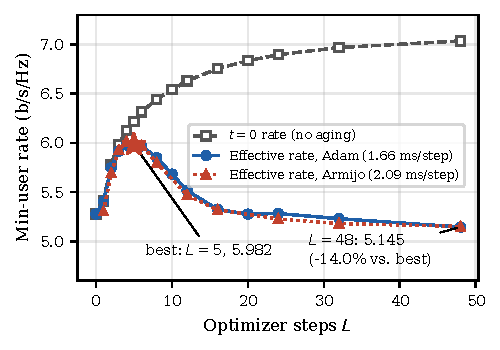
\includegraphics[width=0.92\columnwidth]{figures/fig_intrinsic_optimum.pdf}
\caption{Adım taraması (eskime kümesi). $t=0$ hızı $L$ ile artar; etkin hız $L=4$--$6$'da tepe yapar ve $L=48$'de \%14.0 daha düşüktür. Armijo (adım başına 2.09~ms) aynı biçimi gösterir. $L=0$: 0.05~ms'de SU-best-of (5.276; ölçülen 2.5~ms'sinde 5.272).}
\label{fig:optimum}
\end{figure}

\subsection{Optimumu Tek Bir Sayı Belirler}
\label{sec:res_scaling}
Optimize edilmiş bir gerçekleme adım başına daha hızlı olurdu. Bu nedenle Şekil~\ref{fig:scaling}, Adam'ın adım süresini ölçülen değerin 0.01 ila 3 katı arasında ölçekler, yani $x$'i $2.5\times10^{-4}$'ten $7.5\times10^{-2}$'ye kadar; bu kurulum $x=2.5\times10^{-2}$ noktasındadır ve aynı eksen buradakinden 100 kata kadar daha yavaş ya da 3 kat daha hızlı kullanıcıları da kapsar. En iyi adım sayısı düzenli olarak azalır: en küçük $x$'te 96 adım, ardından 48, 24--32, 12--16, burada 4--6 ve en büyükte 2. En küçük $x$'te yakınsama neredeyse bedavadır ($L=256$'ya kadar koşmanın maliyeti \%1.5, GA \%1.3--1.8); yakınsamanın maliyeti $x\approx 2.5\times10^{-3}$ civarında yaklaşık \%21 ile tepe yapar. $x\ge 2.5\times10^{-2}$ için $L=256$ 200~ms ufkunun ötesindedir; dolayısıyla maliyeti, olsa olsa, olduğundan düşük gösterilmektedir. Bu nedenle yakınsamanın zarar verip vermediği, genel olarak RIS optimizasyonunun değil, rejimin bir özelliğidir. GPU ya da NPU gibi daha hızlı donanım adımı kısaltır ve böylece optimumu kaydırır, ancak onu ortadan kaldırmaz: modelde (Önerme~1) her $x>0$ için bir iç optimum vardır ve ölçümlerde optimum yüz kat daha hızlı bir adıma kadar varlığını sürdürür; orada 96 adımdadır.

Önerme~1'in dayandığı iki yasa da yaklaşık olarak geçerlidir. Eskime kaybı karesele yakındır (her $L$ için $R^2\ge 0.98$, $\tau\le 10$~ms için uydurulmuş) ve $\kappa_L$, $L=1$'de 7.8'den $L=48$'de 25.1'e büyür. Yakınsama açığı kabaca bir kuvvet yasasını izler; $\gamma=0.93$ olmakla birlikte uydurma aralığına bağlı olarak 0.56 ile 1.19 arasında değişir, dolayısıyla öngörülen üs $-0.78$ ile $-0.63$ arasındadır. $L^\star(x)$'in ölçülen eğimi $-0.675$'tir (\%95 GA $-0.692$ ile $-0.655$ arası) ve bu aralığın içindedir; dolayısıyla model üssü ancak yaklaşık $\pm 0.08$ hassasiyetle belirler. Kapalı biçim~\eqref{eq:Lstar}, her $x$'te ölçülen optimumun 1.27 çarpanı içindedir (burada 5.3'e karşı 5). Bu bir örneklem içi denetimdir: $\kappa_L$, optimumların ortaya çıktığı gecikmeler (1.6--10~ms) üzerinde uydurulmuştur. Önerme~1'in dengesi nicel olarak geçerli değildir (oran 0.19 ile 1.65 arasında değişir); dolayısıyla model optimumun nerede bulunduğunu ve neden kaydığını açıklar, iki kaybın nasıl bölüştüğünü değil.

Daha büyük bir $8\times 8$ yüzey ($N=64$) yakınsanmış hızı yükseltir (8.48'e karşı 7.10~b/s/Hz) ancak her adım süresi çarpanında aynı en iyi adım sayısına sahiptir; bu, optimumu doğrular, ama üssü bağımsız olarak doğrulamaz. Adımı bizim kodumuzda yalnızca 1.04 kat daha pahalı olduğundan neredeyse aynı $x$'te yer alır; maliyeti $N$ ile büyüyen bir gerçekleme onu daha az adıma kaydırırdı.

\begin{figure}[t]
\centering
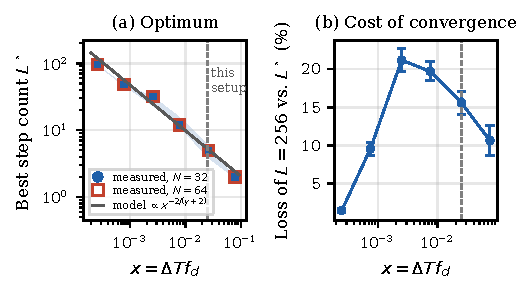
\includegraphics[width=\columnwidth]{figures/fig_step_scaling.pdf}
\caption{Adım süresi ölçülen değerin 0.01 ila 3 katı arasında ölçeklenmiş Adam. (a)~$N=32$ (gölgeli: en iyiden anlamlı ölçüde düşük olmayanlar) ve $N=64$ için en iyi adım sayısı; çizgi: kapalı biçim~\eqref{eq:Lstar}. (b)~$L^\star$ yerine $L=256$'ya kadar koşmanın kaybı ($N=32$), \%95 eşli GA'larla. Kesikli: bu kurulum.}
\label{fig:scaling}
\end{figure}

\subsection{Standartlaştırılmış Hızlar ve Kanal Edinme Gecikmesi}
\label{sec:res_sensitivity}
Tablo~\ref{tab:speeds}, ana ölçümleri aynı senaryolarda, 40~ms'ye kadar 0.5~ms aralıklı bir zaman ızgarasında, standartlardaki kullanıcı hızlarında ve bunlardan daha yüksek iki hızda tekrarlar: 3GPP iç mekân sıcak nokta değerlendirmesinde kullanılan 3~km/h~\cite{3gpp_tr38913}; iç mekân hareketliliğinin değerlendirildiği IMT-2020 yaya sınıfının üst ucu olan 10~km/h~\cite{itu_m2410}; ve yaya sınıfının ötesinde, 18~km/h (5~m/s, araç sınıfında bizim seçimimiz) ile yoğun kentsel değerlendirmenin 30~km/h'i~\cite{3gpp_tr38913,itu_m2410}. Kanal edinme gecikmesi olmadan iki bulgu da---bir optimal adım sayısının varlığı ve yavaş çözücülerin kaybetmesi---her hızda geçerlidir. Optimum 3~km/h'te 8 adımdan 10~km/h'te 3'e, 18~km/h'te 2'ye ve 30~km/h'te 1'e kayar. $L=48$'e kadar koşmanın maliyeti 3~km/h'te \%14.5 (\%95 GA \%13.1--16.1), 10~km/h'te \%10.5'tir (\%9.0--11.9). SU-best-of her hızda koordinat inişinin 0.25--0.42~b/s/Hz, uzun koşulu Adam'ın 0.45--0.69 önündedir ve eşli GA'lar sıfırın üzerindedir (yavaş çözücüler için iyimser değerler). 18 ve 30~km/h'te $L=48$ güvenilir ufkun (60 ve 36~ms) ötesindedir; dolayısıyla bu maliyet yaklaşıktır. 3.43~ms kanal edinme gecikmesiyle optimum 18 ve 30~km/h'te çözümlenemez ve 30~km/h'te SU-best-of ile koordinat inişi artık anlamlı ölçüde farklı değildir. Bu daha ince ızgarada, 1.5~m/s'de $L=4$--$6$ birbirinin \%0.5'i içindedir ve $L=48$'e kadar koşmanın maliyeti \%14.2'dir (ana taramada \%14.0).

\begin{table}[t]
\centering
\caption{Standartlaştırılmış ve daha yüksek kullanıcı hızları (eskime kümesi, kanal edinme gecikmesi yok): eş evrelilik süresi, normalize adım maliyeti, en iyi adım sayısı (\%0.5 içindeki aralık), Adam'ı $L=48$'e kadar koşmanın maliyeti ve $\Delta$: etkin hızda SU-best-of eksi koordinat inişi (b/s/Hz). 0.5~ms'lik bir ızgarada hesaplanmıştır; bu nedenle değerler Tablo~\ref{tab:aging} ve Şekil~\ref{fig:optimum} değerlerinden biraz farklı olabilir. $^\dagger$Güvenilir ufkun ötesinde; yaklaşık.}
\label{tab:speeds}
\footnotesize
\setlength{\tabcolsep}{3pt}
\begin{tabular}{rlrrlrr}
\toprule
km/h & Kaynak & $T_c$ (ms) & $x$ & $L^\star$ & $L{=}48$ & $\Delta$ \\
\midrule
3 & 3GPP~\cite{3gpp_tr38913} & 50.8 & 0.014 & 8 (6--8) & 14.5\% & $+0.27$ \\
5.4 & bu çalışma & 28.2 & 0.025 & 4 (4--6) & 14.2\% & $+0.31$ \\
10 & ITU~\cite{itu_m2410} & 15.2 & 0.046 & 3 & 10.5\% & $+0.25$ \\
18 & bu çalışma, ITU araç & 8.5 & 0.083 & 2 & 8.0\%$^\dagger$ & $+0.42$ \\
30 & ITU, kentsel & 5.1 & 0.139 & 1 & 4.3\%$^\dagger$ & $+0.42$ \\
\bottomrule
\end{tabular}

\end{table}

Konuşlandırılmış bir sistem, optimize etmeden önce pilotlara ve geri beslemeye de zaman harcar. Ana ızgarada, 1--3~m/s'de 0--10~ms'lik bir kanal edinme gecikmesi eklemek optimumu \eqref{eq:marginal} ifadesinin öngördüğü biçimde kaydırır (1.5~m/s'de $L=4$--$6$'dan $L=3$--$4$'e); $T_c/2$'nin üzerindeki gecikmeler dışarıda bırakıldığında (yalnızca 10~ms ile 3~m/s), $L=48$'e kadar koşmanın maliyeti \%2.9--14.7'dir. Optimum yanlış bir hız varsayımını da tolere eder: kullanıcılar 1.8~m/s ile hareket ederken $L$'yi 1.5~m/s için seçmenin maliyeti \%0.5'ten azdır ve ızgaramızdaki hiçbir varsayılan ve gerçek hız çifti \%5.7'den fazlasına mal olmaz.

\emph{Paylaşılan saçılma kazançları.} Fiziksel bir kanalda olduğu gibi tüm BS antenleri için saçıcı başına tek bir kazanç kullanıldığında mutlak hızlar düşer (Tablo~\ref{tab:speeds} ızgarasında 1.5~m/s'de Adam'ın en iyi etkin hızı: 5.984 yerine 5.398~b/s/Hz), ancak bulgular geçerliliğini korur: $L^\star$ 1.5~m/s'de 4--6'da ve 10~km/h'te 3'te kalır, $L=48$'e kadar koşmanın maliyeti sırasıyla \%17.7 (GA \%15.8--19.5) ve \%14.2'dir ve SU-best-of koordinat inişinin ve uzun koşulu Adam'ın önünde kalır (eşli GA'lar sıfırın üzerinde).

\subsection{Periyodik Çalışma: Periyodu Pilotlar Belirler, Kısa Güncellemeler Yeterlidir}
\label{sec:res_tracking}
Tablo~\ref{tab:tracking}, Tanım~3'teki denetleyicinin benzetimini yapar. Ne sıklıkla güncelleme yapılacağına pilot ek yükü karar verir. Bedava pilotlarla, sıcak başlangıçlı iki adımla yapılan art arda güncellemeler en iyisidir (6.36~b/s/Hz); 0.86~ms pilotla en iyi periyot 10--20~ms'dir; 3.43~ms ile, her 80~ms'de bir yapılan güncellemeler (sıcak başlangıç) ve 48 adımlı art arda güncellemeler (soğuk başlangıç) istatistiksel olarak berabedir. Değişmeyen şey, kısa güncellemelerin yeterli olmasıdır: her satırda, en fazla 8 adımlı ve en iyiden anlamlı ölçüde düşük olmayan bir politika vardır. Sıcak başlangıç, pilotlar kısa olduğunda 0.53~b/s/Hz'e kadar kazanç sağlar, 3.43~ms pilotlarla ise anlamlı hiçbir kazanç sağlamaz.

\begin{table}[t]
\centering
\caption{Periyodik yeniden optimizasyon (eskime kümesi): $T_{\mathrm{p}}$ pilot süreleri için en iyi güncelleme periyodu $U$ (ms; b2b = art arda) ve güncelleme başına adım $L$, zaman ortalamalı etkin hızla (b/s/Hz) birlikte. Sıcak$-$soğuk: en iyi iki politikanın eşli farkı; $^\S$anlamlı değil.}
\label{tab:tracking}
\footnotesize
\setlength{\tabcolsep}{5.5pt}
\begin{tabular}{r|rrr|rrr|r}
\toprule
 & \multicolumn{3}{c|}{Soğuk başlangıç} & \multicolumn{3}{c|}{Sıcak başlangıç} & \\
$T_{\mathrm{p}}$ (ms) & $U$ & $L$ & hız & $U$ & $L$ & hız & sıcak$-$soğuk \\
\midrule
0 & b2b & 3 & 5.83 & b2b & 2 & 6.36 & +0.53 \\
0.86 & 20 & 3 & 5.24 & 10 & 3 & 5.51 & +0.28 \\
1.71 & b2b & 48 & 5.08 & 20 & 3 & 5.17 & +0.09 \\
3.43 & b2b & 48 & 4.98 & 80 & 24 & 4.99 & +0.01$^\S$ \\
\bottomrule
\end{tabular}

\end{table}

\subsection{Öğrenilen Bir Güncelleme Kuralı Adım Başına Kazanır ama Milisaniye Başına Kaybeder}
\label{sec:res_reversal}
Bu karşılaştırma, hesaplama verimliliğini yalıtmak için statik kümeyi ve $t=0$ hızlarını kullanır. Eşit adım sayısında öğrenilen kural, her $L\in\{1,2,4,8,16\}$ bütçesinde ayarlanmış Adam'ı yener (Şekil~\ref{fig:eqms}(a)) ve test senaryolarının \%68--84'ünde kazanır. Ancak tek bir öğrenilen adım, 2.7--4.0 Adam adımı kadar zaman alır. Ölçülen zaman ekseninde (Şekil~\ref{fig:eqms}(b)), beş zamanlama turunun her birinde, her öğrenilen yapılandırma hem daha hızlı hem daha iyi olan bir Adam yapılandırması tarafından baskınlanır. Örneğin $L=4$ ile öğrenilen kural 5.285~b/s/Hz için 18.41~ms gerektirirken $L=8$ ile Adam 5.380~b/s/Hz için 13.48~ms gerektirir. Eşit adım sıralaması tamamen tersine döner. Eskime burada dahil edilmemiştir; her çiftte daha yavaş olan öğrenilen yapılandırma olduğundan, eskimenin aradaki farkı açması beklenirdi. Ancak maliyet oranı, bu gerçeklemenin tek bir CPU iş parçacığı üzerindeki bir özelliğidir: ağın matris çarpımlarını Adam'ın adımından daha fazla hızlandıran donanımda bu tersine dönme zayıflayabilir.

\begin{figure*}[t]
\centering
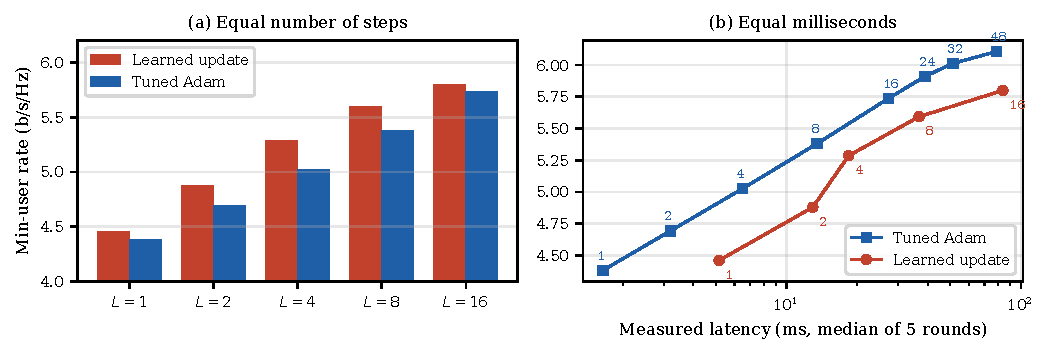
\includegraphics[width=\textwidth]{figures/fig_equal_step_vs_ms.pdf}
\caption{Öğrenilen güncelleme kuralı ile ayarlanmış Adam'ın karşılaştırması (statik test kümesi, 600 senaryo, $t=0$ hızları, tek CPU iş parçacığı). (a)~Eşit adımda öğrenilen kural her bütçede öndedir. (b)~Ölçülen gecikme ekseninde (etiketler: adım sayısı $L$), her öğrenilen yapılandırma Adam eğrisinin altında ve sağında yer alır: baskınlanmıştır.}
\label{fig:eqms}
\end{figure*}

\subsection{Taze Hüzme Varsayımı Önemlidir}
\label{sec:res_beam}
Ana sonuçlar, yalnızca RIS fazı eskirken BS'nin ön kodlayıcısını güncel kanaldan tazelediğini varsayar. Hüzme kümesinde, bunun yerine ön kodlayıcıyı $t=0$ anındaki hâliyle tutmak hızın onlarca milisaniye içinde çökmesine yol açar: $T_c$ anında hız, her faz seçimi için, taze hüzmeye göre 11.7--14.2$\times$ daha düşüktür ve Adam'ın ($L=8$) fazıyla yalnızca 5~ms yaşındaki bir ön kodlayıcı bile hızı 5.228'den 1.736~b/s/Hz'e düşürür (hüzme kümesi hızları Tablo~\ref{tab:aging} ile karşılaştırılabilir değildir). Ön kodlayıcıyı tazelemek ucuzdur (0.12~ms, bir Adam adımından yaklaşık 13 kat kısa), ancak birkaç milisaniyede bir etkin kanal pilotları gerektirir; bunların yayın süresi Bölüm~\ref{sec:res_robust} kapsamında hesaba katılır.

\subsection{Pilotlara, Kestirim Hatasına ve Faz Çözünürlüğüne Dayanıklılık}
\label{sec:res_robust}
Bu denetimler eskime kümesini ve Bölüm~\ref{sec:method} kapsamında yeniden ölçülen gecikmeleri (Adam adımı başına 1.33~ms) kullanır. Yapılandırmalar bağımsız bir hareketlilik çekilişinde (tohum 12) seçilir ve eşli GA'larla raporlanır; $L^\star$ eskime kümesinde okunur.

\emph{Ön kodlayıcı pilotları.} Ön kodlayıcı, veri taşımayan dört pilot sembolünden her $T_{\mathrm{r}}$~ms'de bir tazelendiğinde ($T_{\mathrm{r}}$ yönteme göre seçilir) ve en düşük kullanıcı hızı, pilotlar düşülerek, konuşlandırmadan sonraki $W$~ms boyunca ortalandığında ($\bar{R}_W$), seçilen yapılandırma bedava tazelemeyle 5.21~b/s/Hz'e, 15, 30 ve 60~kHz alt taşıyıcı aralığında ise 3.54, 4.00 ve 4.33~b/s/Hz'e ulaşır ($W=50$~ms, $T_{\mathrm{r}}=1$--2~ms). Bu yapılandırma 6--8 Adam adımı kullanır; 3--20 adım onunla berabedir ve koordinat inişi ile uzun koşulu Adam anlamlı ölçüde geridedir. $W=25$, 50 ve 100~ms için seçilen adım sayıları 5, 6--8 ve 16--20'dir (bedava tazelemeyle 16--24); 100~ms'de, pilotlarla, altı adım 0.02--0.04~b/s/Hz aşağıda kalır. Ancak SU-best-of'a karşı, koordinat inişi (0.70~s sonra, güvenilir ufkun ötesinde, modelin onu kayırdığı bölgede konuşlandırılır) pilotlarla $W=50$~ms'de berabere kalır ve bedava tazelemeyle ya da $W=100$~ms'de 0.09--0.18~b/s/Hz önde olur (15~kHz hariç); onu her pencerede yalnızca ayarlanmış Adam yener.

\emph{Kusurlu kanal bilgisi.} Ortalama kanal gücüne göre $1/(1+\rho)$ güçte kestirim hatasıyla ($\rho$: pilot sinyal-gürültü oranı; 30~dB'de RIS--kullanıcı kanalı için senaryo başına medyan 22.6~dB), faz $t=0$ kestiriminden ve ön kodlayıcı taze bir kestirimden alındığında, en iyi etkin hız 30 ve 20~dB'de 6.08'den 3.54 ve 1.40~b/s/Hz'e düşer (ikincisi, tek başına doğrudan bağlantının değeri olan 1.74'ün altındadır); 10~dB ve altında hızlar sıfıra yakındır ve Adam ile SU-best-of berabedir. Pilotlar da hesaba katıldığında ($\bar{R}_{50}$), Adam 30~dB'de SU-best-of'un 0.05--0.06~b/s/Hz önündedir ve 20~dB'de onunla berabedir; koordinat inişi ve uzun koşulu Adam anlamlı ölçüde geride kalmaya devam eder.

\emph{Ayrık fazlar.} Adam'ın (adım boyu 0.5) ve SU-best-of'un fazlarını hiçbir zaman maliyeti olmadan $2^b$ düzeye yuvarlamak içsel bir optimumu korur ($b=1$, 2, 3 için $L^\star=5$, 6, 6; $L=48$'in maliyeti \%9.5, \%14.1, \%14.9). $2^b$ düzey üzerinde ayrık koordinat inişi (16--501~ms), $b=3$'te ve iki ya da daha fazla taramayla $b=2$'de yuvarlanmış SU-best-of'un anlamlı ölçüde gerisindedir. $b=1$'de tek bir taramayla (16~ms) seçilir: yuvarlanmış SU-best-of'un 0.25~b/s/Hz (GA 0.16--0.33) üzerindedir ve en iyi yuvarlanmış Adam ile berabedir ($-0.04$, GA $-0.11$ ile 0.02 arası).
